\documentclass[a4paper,12pt,oneside,openany]{book}

%%%%%%%%%%%%%%%%%%%%%%%%%%%%%%%%%%%%%%%%%%%%%%%%%%%%%
%%%%%%%%%%%      THESIS PARAMETERS       %%%%%%%%%%%%
%%%%%%%%%%%%%%%%%%%%%%%%%%%%%%%%%%%%%%%%%%%%%%%%%%%%%

% Language Option: "tr" or "eng"                (default: "eng")
% Degree Option: "ms" or "phd"                  (default: "ms")
% For Thesis Monitoring Committee Report: "tmc"
% Bibliography Option: "ieee" or "authoryear"   (default: "ieee")

% Example:   \usepackage[tr, phd, tmc]{ytuthesis}
%            \usepackage[eng, ms]{ytuthesis}
%            \usepackage[tr, ms, authoryear]{ytuthesis}
\usepackage[eng, ms]{ytuthesis}

% this is for algoritm boxes
\usepackage{hyperref}
\usepackage{listings}
\usepackage{xcolor}
\usepackage{makecell}
\usepackage{threeparttable}
 
\definecolor{codegreen}{rgb}{0,0.6,0}
\definecolor{codegray}{rgb}{0.5,0.5,0.5}
\definecolor{codepurple}{rgb}{0.58,0,0.82}
\definecolor{backcolour}{rgb}{0.95,0.95,0.92}
 
\lstdefinestyle{mystyle}{
    backgroundcolor=\color{backcolour},   
    commentstyle=\color{codegreen},
    keywordstyle=\color{magenta},
    numberstyle=\tiny\color{codegray},
    stringstyle=\color{codepurple},
    basicstyle=\ttfamily\footnotesize,
    breakatwhitespace=false,         
    breaklines=true,                 
    captionpos=t,                    
    keepspaces=true,                 
    numbers=left,                    
    numbersep=5pt,                  
    showspaces=false,                
    showstringspaces=false,
    showtabs=false,                  
    tabsize=2,
    xleftmargin=10pt
}
 

\lstset{style=mystyle}

%% this is for adding algoritm boxes into Tables list
\usepackage{hyperref}
\makeatletter
% Grab the old \addcontentsline, which has been already being redefined by hyperref (eventually)
\let\latex@@addcontentsline\addcontentsline 

\AtBeginDocument{%
    \renewcommand{\addcontentsline}[3]{%
  \def\@@zzz{#1}\def\@@zxx{lol}
  \latex@@addcontentsline{%
    \ifx\@@zzz\@@zxx lot\else #1\fi
  }{#2}{#3}%
}

\renewcommand\lstlistingname{Table}
\let\l@lstlisting\l@table
\let\c@lstlisting\c@table
\let\thelstlisting\thetable
\let\ftype@lstlisting\ftype@table
}
\makeatother

%%% for prettier tables
\usepackage{booktabs}
\renewcommand{\arraystretch}{1.2}
\usepackage{colortbl}%
  \newcommand{\myrowcolour}{\rowcolor[gray]{0.925}}
%% \usepackage[table]{xcolor}

%% footnotes for tables
%% source: https://tex.stackexchange.com/a/109471
\usepackage{footnote}
\makesavenoteenv{tabular}
\makesavenoteenv{table}


%%%%%%%%%%%%%%%%%%%%%%%%%%%%%%%%%%%%%%%%%%%%%%%%%%%%%
%%%%%%%%%%%         REFERENCES       %%%%%%%%%%%%%%%%
%%%%%%%%%%%%%%%%%%%%%%%%%%%%%%%%%%%%%%%%%%%%%%%%%%%%%
\addbibresource{references.bib} 



\begin{document}
%%%%%%%%%%%%%%%%%%%%%%%%%%%%%%%%%%%%%%%%%%%%%%%%%%%%%
%%%%%%%%%%%         FRONT PAGES      %%%%%%%%%%%%%%%%
%%%%%%%%%%%%%%%%%%%%%%%%%%%%%%%%%%%%%%%%%%%%%%%%%%%%%
\input {frontPages.tex}


%%%%%%%%%%%%%%%%%%%%%%%%%%%%%%%%%%%%%%%%%%%%%%%%%%%%%
%%%%%%%%%%%%%%%      CHAPTERS     %%%%%%%%%%%%%%%%%%%
%%%%%%%%%%%%%%%%%%%%%%%%%%%%%%%%%%%%%%%%%%%%%%%%%%%%%

\chapter{GİRİŞ}

%\chapter{INTRODUCTION}

\section{Literature Review}
Istanbul is a beautiful city of stunning architecture, history and culture. You'll find ancient and modern colleges, fascinating museums and galleries, and plenty of parks, gardens and green spaces in which to relax. Although the city is spread over a large area, you will have easy reach to anywhere you would like to go thanks to a variety of modern and developed transportation systems diversing from interchangeable rail systems to long-way metrobus lines.

İkinci paragrafa başlamak için iki defa enter'a basıyoruz.

\begin{theorem}
Let $f$ be a function whose derivative exists in every point, then $f$ is 
a continuous function.
\end{theorem}
 
\begin{theorem}[Pythagorean theorem]
\label{pythagorean}
This is a theorema about right triangles and can be summarised in the next 
equation 
\begin{equation}
x^2 + y^2 = z^2
\end{equation}
\end{theorem}

And a consequence of theorem \ref{pythagorean} is the statement in the next 
corollary.
 
\begin{corollary}
There's no right rectangle whose sides measure 3cm, 4cm, and 6cm.
\end{corollary}
 

Unnumbered theorem-like environments are also possible.
 
\begin{remark}
This statement is true, I guess.
\end{remark}
 
And the next is a somewhat informal definition
 
\theoremstyle{definition}
\begin{definition}{Fibration}
A fibration is a mapping between two topological spaces that has the homotopy lifting property for every space $X$.
\end{definition}

\begin{lemma}
Given two line segments whose lengths are $a$ and $b$ respectively there 
is a real number $r$ such that $b=ra$.
\end{lemma}
 
\begin{proof}
To prove it by contradiction try and assume that the statemenet is false,
proceed from there and at some point you will arrive to a contradiction.
\end{proof}

 
You can reference theorems such as \ref{pythagorean} when a label is assigned.
 
\begin{lemma}
Given two line segments whose lengths are $a$ and $b$ respectively there is a 
real number $r$ such that $b=ra$.
\end{lemma}

\section{Objective of the Thesis}
There are two airports in Istanbul. Atatürk Airport is on the European Side of the city, and Sabiha Gökçen Airport is on the Asian Side. As both of the airports are located outside the city centre you may find the taxi fees fairly expensive. The taxi from Atatürk Airport to Yıldız Central Campus will cost around Euro 35-40. In case you arrive at the Sabiha Gökçen Airport, you will need to pay double this amount to get here and you will also have to add the bridge fee to it. Communication with the taxi driver will be much easier if you write down the address and hand it to him.

%Sayfayı \end{landscape} komutuna kadar yatay olarak işler
%\begin{landscape}
\section{Hypothesis}
You may only use this method of transport from the Atatürk Airport. You can easily reach the station by following the “Metro” signs. If you have difficulties, you can easily ask airline staff for directions. In order to get on the metro, you need to buy a token from the counter. You need to use this token to go through the turnstiles in order to get to the train. You can enjoy the journey without getting stressed as you will go from the first station the last station. You can easily come out at the Aksaray Station, the last station, by following the signs. We suggest you get a taxi from here. Your location is not too close to Yıldız Central Campus but it is also not too far. The taxi from here will cost approx. Euro15.
%\end{landscape}
\chapter{DENKLEM, RESİM, ALGORİTMA ÖRNEKLERİ}
Istanbul is a beautiful city of stunning architecture, history and culture. You'll find ancient and modern colleges, fascinating museums and galleries, and plenty of parks, gardens and green spaces in which to relax. Although the city is spread over a large area, you will have easy reach to anywhere you would like to go thanks to a variety of modern and developed transportation systems as well as interchangeable rail systems to long-way metrobus lines.

\begin{figure}[!htbp]
\centering
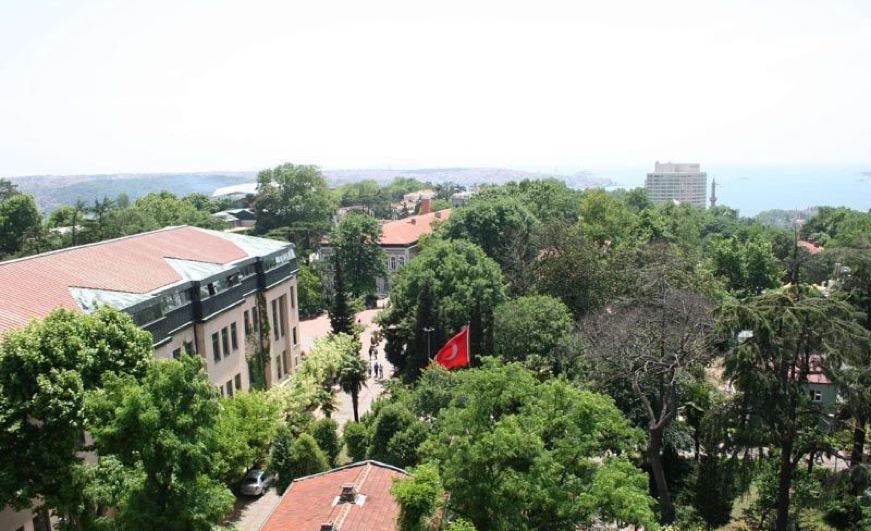
\includegraphics[width=\textwidth]{thesisChapters/images/Picture1.png}
\caption{Landscape design of Yıldız Technical University}
\label{fig:landscape}
\end{figure}

In Figure \ref{fig:landscape}, landscape design of Yıldız Technical University is illustrated.

\section{History}
The stages our university has passed through in its distinguished past are outlined below. Kondüktör Mekteb-i Âlisi/ The Conductors (Technicians) School of Higher Education (1911-1922). The Kondüktör Mekteb-i Âlisi/Conductors (Technicians) School of Higher Education was founded in 1911 in order to meet the “science officer” (known previously as conductors, and today as technicians) requirement of the Municipality Public Works Section. The school was modeled on the syllabus of the “Ecole de Conducteur” and was affiliated with the Ministry of Public Works. Enrolment began on 22 August 1911. Harita ~\ref{fig:itu} de İTÜ haritasıdır.

\begin{map}[!htbp]
\centering
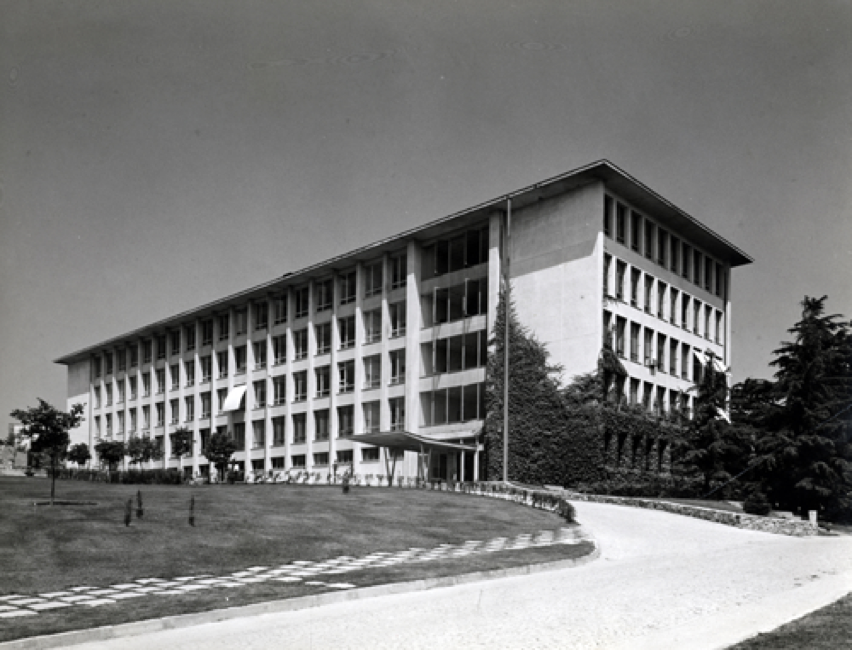
\includegraphics[width=\textwidth]{thesisChapters/images/Picture2}
%\includegraphics[scale=0.6]
\caption{The Istanbul Technical School}
\label{fig:itu}
\end{map}

\textbf{Nafia Fen Mektebi/ The School of Public Works (1922-1937):}  The school’s name was changed to Nafia Fen Mektebi/ School of Public Works in 1922 and the duration of education was increased to 2.5 years in 1926 and 3 years in 1931.

\section{Historical Advancements in the University}

The school was established as an autonomous higher education and research institution with Law no. 1184 of State Engineering and Architectural Academies published on 3 June 1969. 

Law no. 1472 ruled for the closing of special vocational schools in 1971, and engineering schools were affiliated with the Istanbul State Engineering and Architectural Academy.

\subsection{The Yıldız University Period}
The Istanbul State Engineering and Architectural Academy and affiliated schools of engineering and the related faculties and departments of the Kocaeli State Engineering and Architecture Academy and the Kocaeli Vocational School were merged to form Yıldız University with decree law no.41 dated 20 June 1982 and Law no. 2809 dated 30 March 1982 which accepted the decree law with changes.

The new university incorporated the departments of Science-Literature and Engineering, the Vocational School in Kocaeli, a Science Institute, a Social Sciences Institute and the Foreign Languages, Atatürk Principles and the History of Revolution, Turkish Language, Physical Education and Fine Arts departments affiliated with the Rectorate.

\subsection{The Yıldız Technical University Period}
Law no. 3837 dated 3 July 1992 renamed our university Yıldız Technical University. The Engineering Faculty was divided into four faculties and restructured as the Electrical-Electronics, Construction, Mechanical and Chemical-Metallurgy Faculties and also included the Faculty of Economics and Administrative Sciences within its organization. The Kocaeli Faculty of Engineering and the Kocaeli Vocational School were released from our university to be restructured as Kocaeli University. Today our university has 9 Faculties \footnote{2 of these faculties are located at Yildiz Campus, and the other ones are located at Davutpaşa Campus}, 2 Institutes, the Vocational School of Higher Education, the Vocational School for National Palaces and Historical Buildings, the Vocational School for Foreign Languages and more than 20,000 students . 

\begin{figure}[htbp]
\centering
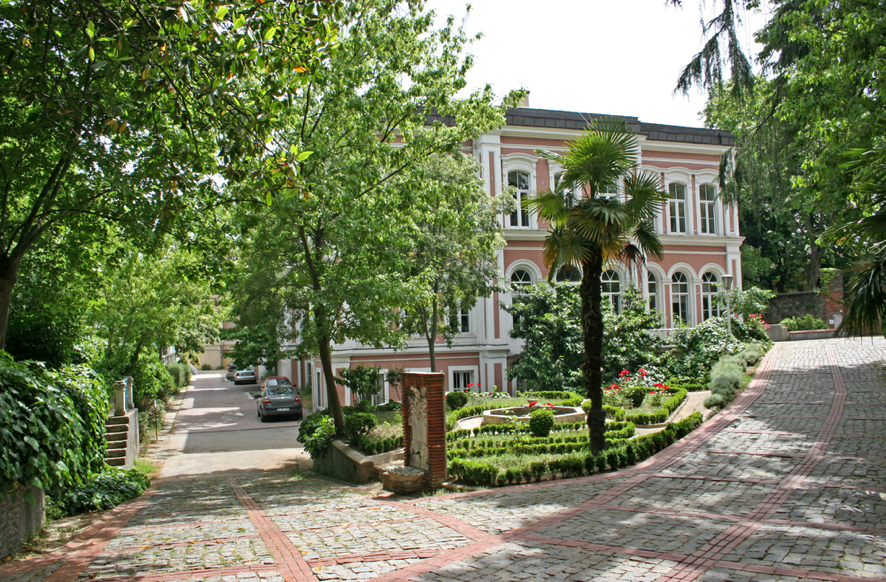
\includegraphics[width=\textwidth]{thesisChapters/images/Picture3}
\caption{Side view of Graduate School of Natural and Applied Sciences, Yıldız Technical University, Çukursaray, İstanbul [10]}
\end{figure}

\subsubsection{Mission}
Our mission is to create a university which pioneers education, scientific research, technological development and artistic work aimed at the progress of society and the increase of the quality of life within an understanding of national and international solidarity; and educates creative, enterprising, questioning and ethical students equipped with universal values, who constantly renew themselves, aim for lifelong learning and are capable of analysis and synthesis.

\begin{equation}
\Delta  l = h \Delta \theta
\end{equation}
\begin{equation}
\frac{\Delta l}{\Delta t} = h \frac{\Delta \theta}{\Delta t}
\end{equation}
\begin{equation}
\lim_{\Delta t \rightarrow 0}\frac{\Delta l}{\Delta t} = \lim_{\Delta t \rightarrow 0} h \frac{\Delta \theta}{\Delta t}
\end{equation}
\begin{equation}
\lim_{\Delta t \rightarrow 0}\frac{\Delta l}{\Delta t} = \frac{dI}{dt}
\end{equation}

Here's more complex formula example.

\subsection{Skip-gram}
Skip-gram metodunda bir kelime girilir ve daha sonra belirli pencere etrafındaki kelimeler tahmin ettirilir. Tek bir girdi değerinden etrafındaki kelimeri çıktı olarak alabiliyoruz. Skip-gram modeli, verilen corpus'a göre her kelimenin kelime vektörlerini eğitir. Cümle içinde bir kelime \textit{(W(t))} verildiğinde,mevcut kelimenin \textit{W(t)} olasılığıyla. skip-gram, yakındaki $w_{i}(t-k\leqslant i\leqslant t + k)$ kelimelerinin \textit{P(W(t+i)|W(t))} olasılıklarını tahmin edebilir.Her sözcük vektörü yakındaki kelimelerin konumlarını yansıtır. Skip-gram modelinin amacı aşağıdaki değeri en üst düzeye çıkarmaktır:

\begin{equation}
    \centering
    E=\frac{1}{n}\sum\limits_{t=1}^{n}{\left(\sum\limits_{-k\le i\le k,i\ne 0}{{{log}_{2}}P(W(t+i)|W(t))} \right)}
\end{equation}


\section{Algoritma gösterimi}

Algoritma örnekleri tablo olarak alınır. Tablo \ref{model}'de görüldüğü üzere programlama diline göre format gösterimi, satır numarası gösterimi mümkündür.

\begin{lstlisting}[language=python, caption=Construction of the Model , label=model]
from keras.datasets import imdb
from keras import models
from keras.callbacks import ModelCheckpoint
from keras import layers
from keras import optimizers
from keras import losses
from keras.callbacks import EarlyStopping, ModelCheckpoint
from keras.models import load_model
import csv
import matplotlib.pyplot as plt
import pandas as pd
import numpy as np
import sys
import argparse

\end{lstlisting}

\section{Tablo örnek}

Tablo \ref{phardesc}'de tablo başlığı boyalı halde gösterilmiştir.

\begin{table}[!ht]
\caption{Cavity Point Features and Pharmacophore Matching Rules}
\centering
\begin{tabular}{l l l l}
\rowcolor{gray!25}
\toprule
\textbf{Property}    &\textbf{Name}  &\textbf{Residue}     &\textbf{Closest Protein Atom} \\ 
\midrule
Hydrophobic(HYD)    &CA   &Gly    &Hydrophobic        \\ 
Aromatic(AR)     &CZ  &Phe    &Aromatic                \\ 
Acceptor(HBA)   &O    &Ala    &Donor                   \\ 
Donor(HBD)      &N   &Ala     &Acceptor      \\ 
Acceptor/Donor(HBAD)  &OG   & Ser      &Acceptor/Donor \\ 
Positive Ionizable(D+)  &NZ   & Lys    &Negative Ionizable    \\ 
Negative Ionizable(A-)  &OD1   & Asp   &Positive Ionizable     \\ 
Null(DU)  &DU   &Cub      &None     \\ 
\bottomrule
\end{tabular}
\label{phardesc}
\end{table}

\chapter{ATIF ÖRNEKLERİ}

Bu tezde IEEE ya da APA stili, kaynakça gösteriminde kullanılmalıdır. "main.tex" isimli dosyada bunu belirtebilirsiniz. Varsayılan ayar IEEE şeklindedir. Eğer APA stilini kullanmak isterseniz:

$usepackage[eng, phd]{ytuthesis}$

satırına 3. parametre olarak authoryear eklemeniz gerekmektedir.

$usepackage[eng, phd, authoryear]{ytuthesis}$ gibi

Kaynak atıfları, noktadan önceki en son öge olmalıdır. Şekil, tablo vs. ye yapılan atıflar, kaynak atıfından önce olmalıdır.

Kaynakları bibtex formatında Google Scholar'dan edinmenizi öneririz. Edindiğiniz bu bilgileri, tezdeki "references.bib" dosyasına yapıştırın.

%Şu an yazdığımız if komutunu KULLANMAYIN. Bu komut sadece ieee ve apa stillerini ayrı ayrı gösterebilmek için kullanılmıştır. IEEE için cite, APA için textcite komutlarını kullanacaksınız. Aşağıdaki ifadelere ve örneklere dikkat edin.

\if@ieeetrue

"Kanser ölümcül bir hastalıktır. Çoğunlukla göğüs, kolon ve kan kanseri tür olarak yaygındır ~\cite{biopsy}. Histopatolojik görüntüler, kanserin erken teşhisinde kullanılan bir veri türü olup Yunanca "Doku hastalıkları bilimi" anlamına gelmektedir ~\cite{mohan2018textbook}. Bu alanda oluşturulan verileri Van Hulse bir konferans bildirisiyle ~\cite{van2007experimental} ve Rao da bir makale çalışmasında incelemiştir ~\cite{xing2016robust}."

\else
"Kanser ölümcül bir hastalıktır.  ~\parencite{biopsy}'ye göre çoğunlukla göğüs, kolon ve kan kanseri tür olarak yaygındır. ~\parencite{mohan2018textbook}'de yazmış olduğu kitabında histopatolojik görüntülerin, kanserin erken teşhisinde kullanılan bir veri türü olup Yunanca "Doku hastalıkları bilimi" anlamına geldiğini belirtmiştir.Bu alanda oluşturulan verileri ~\parencite{van2007experimental, xing2016robust} akademik çalışmalarında incelemiştir." 
\fi

Kaynakça sayfası ve kaynak numaralandırılması, eklediğiniz bilgiler ve yerleri çerçevesinde otomatik olarak oluşturulacaktır.

\section{National Agency }
Currently 2199 higher education institutions in 31 countries are participating in Erasmus. Since the creation of Erasmus in 1987, 1.2 million students have benefited from an Erasmus study period abroad. The Erasmus budget for the year 2004 is more than \euro 187.5 million.

Generally, National Agencies are founded in the participatory countries so as to utilize EU Education and Youth programs by organizing and coordinating activities in cooperation with the relevant parties.
National Agency, a part of State Planning Agency, is responsible for the coordination of the European Union Education Programs in Turkey.

\section{About YTU}
Yıldız Technical University is one of the seven government universities situated in İstanbul besides being the 3rd oldest university of Turkey with its history dating back to 1911.It is regarded as one of the best universities in the country as well. Our university has 10 Faculties, 2 Institutes, the Vocational School of Higher Education, the Vocational School for National Palaces and Historical Buildings, the Vocational School for Foreign Languages and more than 25,000 students. 
As YTU our mission is to create a university which pioneers education, scientific research, technological development and artistic work aimed at the progress of society and the increase of the quality of life within an understanding of national and international solidarity

\begin{table}[!ht]
\caption{Erasmus country codes for different national agencies according to the type of the countries}
\centering
\begin{tabular}{|c|c|c|c|c|c|}
\hline
\textbf{No.} & \textbf{\begin{tabular}[c]{@{}c@{}}National\\ Agencies\end{tabular}}   & \textbf{\begin{tabular}[c]{@{}c@{}}Erasmus\\ Code\end{tabular}} & \textbf{\begin{tabular}[c]{@{}c@{}}ISO\\ Code\end{tabular}} & \textbf{\begin{tabular}[c]{@{}c@{}}NA \\ Identifier\end{tabular}} & \textbf{\begin{tabular}[c]{@{}c@{}}Type of\\ Country\end{tabular}} \\ \hline
1            & Austria                                                                & A                                                               & AT                                                          & AT                                                                & EU                                                                 \\ \hline
2            & \begin{tabular}[c]{@{}c@{}}Belgium\\ (Flemish\\ speaking)\end{tabular} & B                                                               & BE                                                          & BEFL                                                              & EU                                                                 \\ \hline
3            & \begin{tabular}[c]{@{}c@{}}Belgium\\ (French\\ speaking)\end{tabular}  & B                                                               & BE                                                          & BEFR                                                              & EU                                                                 \\ \hline
4            & Bulgaria                                                               & BG                                                              & BG                                                          & BG                                                                & Candidate                                                          \\ \hline
5            & \begin{tabular}[c]{@{}c@{}}Czech\\ Republic\end{tabular}               & CZ                                                              & CZ                                                          & CZ                                                                & EU                                                                 \\ \hline
6            & Cyprus                                                                 & CY                                                              & CY                                                          & CY                                                                & EU                                                                 \\ \hline
7            & Denmark                                                                & DK                                                              & DK                                                          & DK                                                                & EU                                                                 \\ \hline
8            & Estonia                                                                & EE                                                              & EE                                                          & EE                                                                & EU                                                                 \\ \hline
9            & Germany                                                                & D                                                               & DE                                                          & DE                                                                & EU                                                                 \\ \hline
10           & Spain                                                                  & E                                                               & ES                                                          & ES                                                                & EU                                                                 \\ \hline
11           & Finland                                                                & SF                                                              & FI                                                          & FI                                                                & EU                                                                 \\ \hline
12           & France                                                                 & F                                                               & FR                                                          & FR                                                                & EU                                                                 \\ \hline
13           & Greece                                                                 & G                                                               & GR                                                          & GR                                                                & EU                                                                 \\ \hline
14           & Hungary                                                                & HU                                                              & HU                                                          & HU                                                                & EU                                                                 \\ \hline
15           & Iceland                                                                & IS                                                              & IS                                                          & IS                                                                & EEA                                                                \\ \hline
16           & Ireland                                                                & IRL                                                             & IE                                                          & IE                                                                & EU                                                                 \\ \hline
17           & Italy                                                                  & I                                                               & IT                                                          & IT                                                                & EU                                                                 \\ \hline
18           & Latvia                                                                 & LV                                                              & LV                                                          & LV                                                                & EU                                                                 \\ \hline
19           & Liechtenstein                                                          & FL                                                              & LI                                                          & LI                                                                & EEA                                                                \\ \hline
20           & Lithuania                                                              & LT                                                              & LT                                                          & LT                                                                & EU                                                                 \\ \hline
21           & Luxembourg                                                             & LUX                                                             & LU                                                          & LU                                                                & EU                                                                 \\ \hline
22           & Malta                                                                  & MT                                                              & MT                                                          & MT                                                                & EU                                                                 \\ \hline
23           & Netherlands                                                            & NL                                                              & NL                                                          & NL                                                                & EU                                                                 \\ \hline
24           & Norway                                                                 & N                                                               & NO                                                          & NO                                                                & EEA                                                                \\ \hline
25           & Poland                                                                 & PL                                                              & PL                                                          & PL                                                                & EU                                                                 \\ \hline
26           & Portugal                                                               & P                                                               & PT                                                          & PT                                                                & EU                                                                 \\ \hline
27           & Romania                                                                & RO                                                              & RO                                                          & RO                                                                & Candidate                                                          \\ \hline
28           & \begin{tabular}[c]{@{}c@{}}Slovak\\ Republic\end{tabular}              & SK                                                              & SK                                                          & SK                                                                & EU                                                                 \\ \hline
29           & Slovenia                                                               & SI                                                              & SI                                                          & SI                                                                & EU                                                                 \\ \hline
30           & Sweden                                                                 & S                                                               & SE                                                          & SE                                                                & EU                                                                 \\ \hline
\end{tabular}
\end{table}


\section{Application Procedure}
You are expected to attach the following documents to the online application module.

\begin{itemize}
%\setlength{\itemsep}{0pt}
\item Application form
\item Learning agreement
\item Dormitory request form 
\item Signed documents
\item ID Card
\end{itemize}

\section{Money Exchange}
The most convenient way to get money  in Turkey is by using your home bank ATM/ cash card or a credit card in a Turkish ATM/ bancomat/ cash machine.

\begin{table}[!ht]
\caption{Area codes for different subjects}
\centering
\begin{tabular}{|c|c|}
\hline
\textbf{Area Code} & \textbf{Subject}      \\ \hline
1                  & Agricultural sciences \\ \hline
2                  & Culture               \\ \hline
3                  & Economics             \\ \hline
4                  & Technology            \\ \hline
5                  & Horticulture          \\ \hline
6                  & Fisheries             \\ \hline
7                  & Forestry              \\ \hline
8                  & Animal                \\ \hline
9                  & Tropical Agriculture  \\ \hline
10                 & Others                \\ \hline
\end{tabular}
\end{table}

But if you want to exchange cash, plenty of places will do it for you. Currency Exchange Offices  are found in tourist and market areas. They offer better exchange rates than most banks, and may or may not charge a commission. Offices in market areas tend to offer better exchange rates than those in tourist areas. Shop around for the best rate and the lowest (or no) commission.

\section{After a Car Accident}
The following is a step-by-step guide on what to do if you are involved in a traffic accident in Turkey.
From 1 April 2008 it is no longer necessary to call the police to the scene of an accident in the following circumstances:

\begin{itemize}
\item When - the accident involves two or more vehicles
\item Where there is only material damage to vehicles
\item When no one is injured or killed
\end{itemize}

Where all concerned parties agree to the cause and who is liable for the accident and providing each driver completes the correct form and all parties involved sign each form, including witnesses if any. 

You should then submit the form to your insurance company who will use the form in conjunction with the other insurance companies concerned to settle liability. (For more details about how to access the form and instructions how to complete the form, please look at the end of this document.)

If agreement cannot be reached, you should immediately call 155 for Traffic Police assistance and follow the guide below:
Do Not Move Your Vehicle from the point of impact unless invited to do so by the traffic police or gendarme.

It is not advisable to accept an offer of financial settlement from the other parties involved. Wait for the police to arrive.
Once the police arrive, you will be breathalyses and asked to produce your driving license and logbook. A preliminary report of the accident will be compiled by the police at the scene of the accident. Only when this report has been made, should you move your vehicle.  It can take half an hour for the police to arrive at the scene of an accident. Do not move your vehicle.

It is essential to obtain the result of the breathalyzer test and the official police report in order to make a successful insurance claim. You will be asked to collect this within three days from the District Police Station.

This leaflet has been prepared by the British Embassy in Ankara for the convenience of enquirers.  Although all care has not been taken in its production, neither Her Majesty's Government nor any Consular Official in the British Embassy in Ankara takes any responsibility for its precise accuracy or for the consequences of any action taken in accordance with its contents.
\chapter{RESULTS AND DISCUSSION}
%Teziniz türkçe ise üst satırı silip aşağıdaki satırı aktif hale getiriniz.
%\chapter{SONUÇ VE ÖNERİLER}

Once you have opened this page you will either have to log in if you are already registered, or register if this is your first visit to this page. When you first register, an e-mail will be automatically sent to you confirming your registration and giving you your password. Once you have logged in you will be able to access the registration form, and you should enter all their details.

Please note that when you have entered your university code and the name of your department, only information which is relevant to your university and department, and which is covered by the relevant bilateral agreement will be displayed.

When you have completed the form, you will find at the bottom of the page a button called 'Attach Files'. This provides a link to where you can attach your completed university application form and Learning Agreement. If you have any special conditions or modifications to the Learning Agreement, you have to contact with your relevant departmental coordinator.

When you are finished, click 'Save' and then 'Send', in order the forms to be sent to this office. Once we have your completed forms we can pass them on to your coordinator here in Yıldız Technical University. Please note that The EU Office cannot make any changes to their form once it has been submitted. Once an understanding has been reached by the coordinators about their application, a Letter of Invitation will be prepared and sent to you.



%%%%%%%%%%%%%%%%%%%%%%%%%%%%%%%%%%%%%%%%%%%%%%%%%%%%%
%%%%%%%%%%%         REFERENCES       %%%%%%%%%%%%%%%%
%%%%%%%%%%%%%%%%%%%%%%%%%%%%%%%%%%%%%%%%%%%%%%%%%%%%%

%% for articles, there's no url entry in .bib file, otherwise, References will show "[Online] Available:" info redundantly.
\newpage
\addcontentsline{toc}{chapter}{\bibName}
\singlespacing
\printbibliography[title={\bibName}]

%%%%%%%%%%%%%%%%%%%%%%%%%%%%%%%%%%%%%%%%%%%%%%%%%%%%%
%%%%%%%%%%%%%%%      APPENDICES     %%%%%%%%%%%%%%%%%
%%%%%%%%%%%%%%%%%%%%%%%%%%%%%%%%%%%%%%%%%%%%%%%%%%%%%

\newpage\appendix

 \chapter{ERASMUS POLICY}
Yıldız Technical University is a major public comprehensive teaching and research university with high aspirations. It has devoted itself to a leading role in contributing through partnerships to socio-cultural and socioeconomic developments at the international level. It has had three years of experiences of participating in the ERASMUS program and its delivery of student and staff mobility has generally been above the national average for Turkey. We are also interested in the programs of LLP such as Comenius, Grundtvig, Leonardo da Vinci. We are going to consider organizing or participating in IP, CD or Thematic Network in the near future. Within the context of the Erasmus Program2007 – 2013, it is aimed to provide students, faculty and staff with more effective research, teaching, and service. With the Erasmus activities, we try to assess where we stood in the past, where we stand today and where we are going to stand in the future, comparing our current position with our peers. With respect to the objectives of the institutionalization of Erasmus student and staff mobility, we try to make our students and our academic staff benefit educationally, linguistically and culturally from the experience of learning in other European countries. We aim to mobilize 2.5 \% of our students and 1.5\% of teaching staff, by the year 2011. We will focus on the technical areas and near and new EU countries because of the exchanging our experiences.

\section{After a Car Accident}
The following is a step-by-step guide on what to do if you are involved in a traffic accident in Turkey.
From 1 April 2008 it is no longer necessary to call the police to the scene of an accident in the following
 
 
 
% \chapter{ERASMUS COUNTRY CODES}

In Table \ref{tab:tableArea}, the area codes for different subjects are listed. The first column of the Table \ref{tab:tableArea} shows the name of the country and the other columns are for the codes of these countries.  
\begin{table}[!ht]
\caption{Area codes for different subjects}
\label{tab:tableArea}

\centering
\begin{tabular}{|c|c|c|c|c|}
\hline
\textbf{Country} & \textbf{Code 1} & \textbf{Code 2} & \textbf{Code 3} & \textbf{Code 4}                                                     \\ \hline
Cyprus           & CY              & CY              & CY              & EU                                                                  \\ \hline
Denmark          & DK              & DK              & DK              & EU                                                                  \\ \hline
Estonia          & EE              & EE              & EE              & EU                                                                  \\ \hline
Germany          & D               & DE              & DE              & EU                                                                  \\ \hline
Spain            & E               & ES              & ES              & EU                                                                  \\ \hline
Finland          & SF              & FI              & FI              & EU                                                                  \\ \hline
France           & F               & FR              & FR              & EU                                                                  \\ \hline
Greece           & G               & GR              & GR              & EU                                                                  \\ \hline
Hungary          & HU              & HU              & HU              & EU                                                                  \\ \hline
Iceland          & IS              & IS              & IS              & EEA                                                                 \\ \hline
Ireland          & IRL             & IE              & IE              & EU                                                                  \\ \hline
Italy            & I               & IT              & IT              & EU                                                                  \\ \hline
Latvia           & LV              & LV              & LV              & EU                                                                  \\ \hline
Liechtenstein    & FL              & LI              & LI              & EEA                                                                 \\ \hline
Slovak Republic  & SK              & SK              & SK              & EU                                                                  \\ \hline
Slovenia         & SI              & SI              & SI              & EU                                                                  \\ \hline
Sweden           & S               & SE              & SE              & EU                                                                  \\ \hline
United Kingdom   & UK              & UK              & UK              & EU                                                                  \\ \hline
Turkey           & TR              & TR              & TR              & Candidate                                                           \\ \hline
Other            & ----            & XX              & ----            & \begin{tabular}[c]{@{}c@{}}Non-participating\\ country\end{tabular} \\ \hline
\end{tabular}
\end{table}

%%%%%%%%%%%%%%%%%%%%%%%%%%%%%%%%%%%%%%%%%%%%%%%%%%%%%
%%%%%%%%%%%     PUBLICATIONS FROM THESIS     %%%%%%%%
%%%%%%%%%%%%%%%%%%%%%%%%%%%%%%%%%%%%%%%%%%%%%%%%%%%%%

%% \ifnum\tmc=0
%% \newpage
%% \addcontentsline{toc}{chapter}{\cvpub}
%% \chapter*{\cvpub}

%Örnekte belirtildiği şekilde e-mail adresinizi yazınız.
\hfill \textbf{\cvcontact:} info@info.com.tr

%%%%%%%%%%%%%%%%%%%%%%%%%%%%%%%%%%%%%%%%%%%%%
%%%%%%%%%%%% TEZİNİZDEN ÜRETİLMİŞ %%%%%%%%%%%
%%%%%%%% DERGİ YAYINLARINIZI YAZINIZ %%%%%%%%
%%%%%%%%%%%%%%%%%%%%%%%%%%%%%%%%%%%%%%%%%%%%%
% Ekleyeceğiniz dergi yayını yoksa aşağıdaki 5 satırı siliniz.
\section*{\cvpapers}
\begin{enumerate}
\item Paper 1
\item Paper 2
\end{enumerate}


%%%%%%%%%%%%%%%%%%%%%%%%%%%%%%%%%%%%%%%%%%%%%
%%%%%%%%%%%% TEZİNİZDEN ÜRETİLMİŞ %%%%%%%%%%%
%%%%%% KONFERANS YAYINLARINIZI YAZINIZ %%%%%%
%%%%%%%%%%%%%%%%%%%%%%%%%%%%%%%%%%%%%%%%%%%%%
% Ekleyeceğiniz konferans yayını yoksa aşağıdaki 5 satırı siliniz.
\section*{\cvconf}
\begin{enumerate}
\item Conference 1
\item Conference 2
\end{enumerate}


%%%%%%%%%%%%%%%%%%%%%%%%%%%%%%%%%%%%%%%%%%%%%
%%%%%%%%%%%% TEZİNİZDEN ÜRETİLMİŞ %%%%%%%%%%%
%%%%%%%%%%% KİTAPLARINIZI YAZINIZ %%%%%%%%%%%
%%%%%%%%%%%%%%%%%%%%%%%%%%%%%%%%%%%%%%%%%%%%%
% Ekleyeceğiniz kitap yayını yoksa aşağıdaki 5 satırı siliniz.
\section*{\cvbooks}
\begin{enumerate}
\item Book 1
\item Book 2
\end{enumerate}


%%%%%%%%%%%%%%%%%%%%%%%%%%%%%%%%%%%%%%%%%%%%%
%%%%%%%%%%%% TEZİNİZDEN ÜRETİLMİŞ %%%%%%%%%%%
%%%%%%%%%%% PROJELERİNİZİ YAZINIZ %%%%%%%%%%%
%%%%%%%%%%%%%%%%%%%%%%%%%%%%%%%%%%%%%%%%%%%%%
% Ekleyeceğiniz proje yoksa aşağıdaki 5 satırı siliniz.
\section*{\cvprojects}
\begin{enumerate}
\item Project 1
\item Project 2
\end{enumerate}


%%%%%%%%%%%%%%%%%%%%%%%%%%%%%%%%%%%%%%%%%%%%%
%%%%%%%%%%%% TEZİNİZDEN ÜRETİLMİŞ %%%%%%%%%%%
%%%%%%%%%%% ÖDÜLLERİNİZİ YAZINIZ %%%%%%%%%%%%
%%%%%%%%%%%%%%%%%%%%%%%%%%%%%%%%%%%%%%%%%%%%%
% Ekleyeceğiniz ödül yoksa aşağıdaki 5 satırı siliniz.
\section*{\cvawards}
\begin{enumerate}
\item Award 1
\item Award 2
\end{enumerate}
%% \fi

\end{document}
